\PassOptionsToPackage{prologue,dvipsnames}{xcolor}
\PassOptionsToPackage{colorlinks=true,linkcolor=Dandelion,urlcolor=magenta,citecolor=violet, hyperfootnotes=true}{hyperref}
\documentclass[aspectratio=169]{beamer}
\usepackage[english]{babel}
\usepackage[utf8]{inputenc}
\usepackage[T1]{fontenc}
\usepackage{csquotes}
\usepackage{color}
\usepackage{float}
\usepackage{multido}
\usepackage{multirow}
\usepackage{array}
\usepackage{enumerate}
\usepackage{booktabs}
\usepackage{indentfirst}
\usepackage[style=alphabetic,maxcitenames=1]{biblatex}
\usepackage{setspace}
\usepackage{calligra}
\usepackage{subcaption}
\usepackage{textpos}
\usepackage{pgfpages}

\usepackage{amsmath,amsfonts,amssymb,amsthm,mathtools,mathrsfs}


\renewcommand<>{\emph}[1]{{\color{Bittersweet}{\only#2{\itshape}#1}}}

\renewcommand*{\bibfont}{\scriptsize}

% TodoNotes and inline notes in fancy boxes
\usepackage{todonotes}
\usepackage{tcolorbox}

% quiver style
\usepackage{tikz-cd}
% `calc` is necessary to draw curved arrows.
\usetikzlibrary{calc}
% `pathmorphing` is necessary to draw squiggly arrows.
\usetikzlibrary{decorations.pathmorphing}

% A TikZ style for curved arrows of a fixed height, due to AndréC.
\tikzset{curve/.style={settings={#1},to path={(\tikztostart)
                    .. controls ($(\tikztostart)!\pv{pos}!(\tikztotarget)!\pv{height}!270:(\tikztotarget)$)
                    and ($(\tikztostart)!1-\pv{pos}!(\tikztotarget)!\pv{height}!270:(\tikztotarget)$)
                    .. (\tikztotarget)\tikztonodes}},
    settings/.code={\tikzset{quiver/.cd,#1}
            \def\pv##1{\pgfkeysvalueof{/tikz/quiver/##1}}},
    quiver/.cd,pos/.initial=0.35,height/.initial=0}

% TikZ arrowhead/tail styles.
\tikzset{tail reversed/.code={\pgfsetarrowsstart{tikzcd to}}}
\tikzset{2tail/.code={\pgfsetarrowsstart{Implies[reversed]}}}
\tikzset{2tail reversed/.code={\pgfsetarrowsstart{Implies}}}
% TikZ arrow styles.
\tikzset{no body/.style={/tikz/dash pattern=on 0 off 1mm}}

% useful macro for class
\newcommand{\at}[3]{\left.#1\right\vert_{#2}^{#3}}
\newcommand\quotient[2]{
    \mathchoice
    {% \displaystyle
        \text{\raise1ex\hbox{$#1$}\Big/\lower1ex\hbox{$#2$}}%
    }
    {% \textstyle
        #1\,/\,#2
    }
    {% \scriptstyle
        #1\,/\,#2
    }
    {% \scriptscriptstyle
        #1\,/\,#2
    }
}

\newcommand{\identity}{\mathrm{id}}
\newcommand{\Homomorphism}{\mathrm{Hom}}
\newcommand{\Morphism}{\mathrm{Mor}}
\newcommand{\Object}{\mathrm{Ob}}
\newcommand{\True}{\textsf{True}}
\newcommand{\T}{\textsf{T}}
\newcommand{\False}{\textsf{False}}
\newcommand{\F}{\textsf{F}}
\newcommand{\act}{\rotatebox[origin=c]{-180}{\(\,\circlearrowright\,\)}}

\usepackage{physics}
\usepackage{complexity}

\DeclareMathOperator{\im}{Im}
\DeclareMathOperator{\sgn}{sgn}
\DeclareMathOperator{\Int}{Int}
\DeclareMathOperator{\diag}{diag}
\DeclareMathOperator{\dom}{dom}
\DeclareMathOperator{\OPT}{\textsf{OPT}}
\DeclareMathOperator*{\argmax}{arg\,max}
\DeclareMathOperator*{\argmin}{arg\,min}
\DeclareMathOperator{\Var}{Var}
\DeclareMathOperator{\Cov}{Cov}

\let\implies\Rightarrow
\let\impliedby\Leftarrow
\let\iff\Leftrightarrow

\usepackage{stmaryrd} % for \lightning
\newcommand\conta{\scalebox{1.1}{\(\lightning\)}}

\usepackage{bm}
\usepackage{bbm}

% figure support
\usepackage{import}
\usepackage{xifthen}
\usepackage{pdfpages}
\usepackage{transparent}
\newcommand{\incfig}[2][\columnwidth]{%
    \def\svgwidth{#1}
    \import{Figures/}{#2.pdf_tex}
}

\newtheorem{intuition}{Intuition}
\AtBeginEnvironment{intuition}{%
    \setbeamercolor{block title}{use=example text,fg=white,bg=VioletRed}
    \setbeamercolor{block body}{parent=normal text,use=block title example,bg=VioletRed!20!white}
}

\newtheorem{remark}{Remark}
\AtBeginEnvironment{remark}{%
    \setbeamercolor{block title}{use=example text,fg=white,bg=Orchid}
    \setbeamercolor{block body}{parent=normal text,use=block title example,bg=Orchid!20!white}
}

\newtheorem{prev}{As previously seen}
\AtBeginEnvironment{prev}{%
    \setbeamercolor{block title}{use=example text,fg=white,bg=gray}
    \setbeamercolor{block body}{parent=normal text,use=block title example,bg=gray!20!white}
}

\newtheorem{assumption}{Assumption}
\AtBeginEnvironment{assumption}{%
    \setbeamercolor{block title}{use=example text,fg=white,bg=Purple}
    \setbeamercolor{block body}{parent=normal text,use=block title example,bg=Purple!20!white}
}

\newtheorem{observe}{Observe}
\AtBeginEnvironment{observe}{%
    \setbeamercolor{block title}{use=example text,fg=white,bg=Purple}
    \setbeamercolor{block body}{parent=normal text,use=block title example,bg=Purple!20!white}
}

\newtheorem{goal}{Goal}
\AtBeginEnvironment{goal}{%
    \setbeamercolor{block title}{use=example text,fg=white,bg=Salmon}
    \setbeamercolor{block body}{parent=normal text,use=block title example,bg=Salmon!20!white}
}

\makeatletter
\let\@@magyar@captionfix\relax
\makeatother


% Corner logo on each slide (add your institution logo to Figures/logo/ and uncomment):
% \addtobeamertemplate{frametitle}{}{
%     \begin{textblock*}{100mm}(0.85\textwidth,-1cm)
%         \includegraphics[height=1cm]{Figures/logo/logo.png}
%     \end{textblock*}}

\definecolor{themecolor}{RGB}{20,49,95}
\mode<presentation>
{
    \usetheme{Madrid}      % or try Darmstadt, Madrid, Warsaw, ...
    \usecolortheme[named=themecolor]{structure} % or try albatross, beaver, crane, ...
    \usefonttheme{default}  % or try serif, structurebold, ...
    \setbeamertemplate{navigation symbols}{}
    \setbeamertemplate{caption}[default]
    \setbeamertemplate{items}[default]
    \setbeamertemplate{section in toc}[ball unnumbered]
}

% Footline: title -- author -- page number (no institute, no date), unified navy bar
\setbeamercolor{title in head/foot}{fg=white,bg=themecolor}
\setbeamercolor{author in head/foot}{fg=white,bg=themecolor}
\setbeamercolor{date in head/foot}{fg=white,bg=themecolor}
\setbeamertemplate{footline}{
    \leavevmode%
    \hbox{%
    \begin{beamercolorbox}[wd=.4\paperwidth,ht=2.25ex,dp=1ex,left,leftskip=2ex]{title in head/foot}%
        \usebeamerfont{title in head/foot}\color{white}{\hypersetup{linkcolor=white}\insertshorttitle}
    \end{beamercolorbox}%
    \begin{beamercolorbox}[wd=.4\paperwidth,ht=2.25ex,dp=1ex,center]{author in head/foot}%
        \usebeamerfont{author in head/foot}\color{white}\insertshortauthor
    \end{beamercolorbox}%
    \begin{beamercolorbox}[wd=.2\paperwidth,ht=2.25ex,dp=1ex,right,rightskip=2ex]{date in head/foot}%
        \usebeamerfont{date in head/foot}\color{white}\insertframenumber/\inserttotalframenumber
    \end{beamercolorbox}}%
    \vskip0pt%
}
\let\oldfootnote\footnote
\renewcommand\footnote[1][]{\oldfootnote[frame,#1]}
\parskip=10pt
\newenvironment<>{proofs}[1][\proofname]{%
    \par
    \def\insertproofname{#1.}%
    \usebeamertemplate{proof begin}#2}
{\usebeamertemplate{proof end}}
\makeatother

% Titlepage logo
\titlegraphic{
\includegraphics[height=1cm]{Figures/logo/umd-seal.png}}

% Title page: move the subtitle out of the navy title box, below it.
\setbeamercolor{subtitle}{fg=themecolor}
\makeatletter
\setbeamertemplate{title page}{
    \vbox{}
    \vfill
    \begingroup
        \centering
        \begin{beamercolorbox}[sep=8pt,center,colsep=-4bp,rounded=true,shadow=true]{title}
            \usebeamerfont{title}\inserttitle\par
        \end{beamercolorbox}%
        \ifx\insertsubtitle\@empty%
        \else%
            \vskip0.35em%
            {\usebeamerfont{subtitle}\usebeamercolor[fg]{subtitle}\insertsubtitle\par}%
        \fi%
        \vskip0.5em\par
        \begin{beamercolorbox}[sep=6pt,center,colsep=-4bp,rounded=true,shadow=true]{author}
            \usebeamerfont{author}\insertauthor
        \end{beamercolorbox}
        \begin{beamercolorbox}[sep=6pt,center,colsep=-4bp,rounded=true,shadow=true]{institute}
            \usebeamerfont{institute}\insertinstitute
        \end{beamercolorbox}
        \vskip0.3em
        {\usebeamercolor[fg]{titlegraphic}\inserttitlegraphic\par}
        \ifx\committeelist\@undefined%
        \else%
            \vskip0.3em%
            {\tiny\color{themecolor}Committee: \committeelist\par}%
        \fi%
        \begin{beamercolorbox}[sep=6pt,center,colsep=-4bp,rounded=true,shadow=true]{date}
            \usebeamerfont{date}\insertdate
        \end{beamercolorbox}
    \endgroup
    \vfill
}
\makeatother

\title[Localized, Edit, and Unlearn in Foundational Models]{Localize, Edit, Unlearn: Structural Interventions\\and Data-Level Control in Foundation Models}
\subtitle{Ph.D. Thesis Defense}
\author{Keivan Rezaei}
\date{September 17, 2026}
\newcommand{\committeelist}{Prof.\ Soheil Feizi (Chair) \textbullet\ Prof.\ Mohammadtaghi Hajiaghayi (Co-Chair) \textbullet\ Prof.\ Sarah Wiegreffe \textbullet\ Prof.\ David Jacobs \textbullet\ Prof.\ Maria K. Cameron}

\addbibresource{reference.bib}

\begin{document}

\begin{frame}
    \titlepage
\end{frame}

\begin{frame}{Table of Content}
    \tableofcontents[hideallsubsections]
\end{frame}

\AtBeginSubsection[]{\begin{frame}\frametitle{Table of Content}\tableofcontents[currentsection,currentsubsection,subsectionstyle=show/shaded/hide]\end{frame}}

\section{Introduction}
\begin{frame}{Roadmap}
    \roadmap{1}
\end{frame}

\begin{frame}{Generative AI: 2022 -- Now}
    \begin{columns}[T,onlytextwidth]
        \column{0.492\textwidth}
        \begin{genbox}{Text-to-Image Models}
            \footnotesize
            \renewcommand{\arraystretch}{1.22}
            \begin{tabular}{@{}l@{\;}c@{\;}l@{}}
                \genyear{2022} & \genicon{openai.pdf}      & \textbf{\dalle{} 2} \genmaker{-- OpenAI}          \\
                \genyear{2022} & \genicon{google.pdf}      & \textbf{Imagen} \genmaker{-- Google}              \\
                \genyear{2022} & \genicon{stabilityai.png} & \textbf{Stable Diffusion} \genmaker{-- Stability} \\
                \genyear{2022} & \genicon{midjourney.pdf}  & \textbf{Midjourney}                                \\
                \genyear{2023} & \genicon{stabilityai.png} & \textbf{SDXL} \genmaker{-- Stability}             \\
                \genyear{2023} & \genicon{openai.pdf}      & \textbf{\dalle{} 3} \genmaker{-- OpenAI}          \\
                \genyear{2024} & \genicon{stabilityai.png} & \textbf{Stable Diffusion 3} \genmaker{-- Stability} \\
                \genyear{2024} & \genicon{google.pdf}      & \textbf{Imagen 3} \genmaker{-- Google}            \\
            \end{tabular}
        \end{genbox}

        \column{0.492\textwidth}
        \begin{genbox}{Large Language Models}
            \footnotesize
            \renewcommand{\arraystretch}{1.22}
            \begin{tabular}{@{}l@{\;}c@{\;}l@{}}
                \genyear{2022} & \genicon{openai.pdf}       & \textbf{ChatGPT} \genmaker{-- OpenAI}     \\
                \genyear{2023} & \genicon{openai.pdf}       & \textbf{GPT-4} \genmaker{-- OpenAI}       \\
                \genyear{2023} & \genicon{anthropic.pdf}    & \textbf{Claude} \genmaker{-- Anthropic}   \\
                \genyear{2023} & \genicon{meta.pdf}         & \textbf{Llama 2} \genmaker{-- Meta}       \\
                \genyear{2023} & \genicon{googlegemini.pdf} & \textbf{Gemini} \genmaker{-- Google}      \\
                \genyear{2024} & \genicon{meta.pdf}         & \textbf{Llama 3} \genmaker{-- Meta}       \\
                \genyear{2025} & \genicon{deepseek.pdf}     & \textbf{DeepSeek-R1} \genmaker{-- DeepSeek} \\
                \genyear{2025} & \genicon{openai.pdf}       & \textbf{GPT-5} \genmaker{-- OpenAI}       \\
            \end{tabular}
        \end{genbox}
    \end{columns}
    \vspace{0.8em}
    \begin{center}
        \small Two paradigms, one common ingredient:
        \textcolor{themecolor}{\textbf{web-scale training data}} baked irreversibly into the weights.
    \end{center}
\end{frame}

\begin{frame}{Text-to-Image: Diffusion}
    \begin{center}
        \begin{tabular}{@{}c@{\;}c@{\;}c@{\;}c@{\;}c@{\;}c@{\;}c@{}}
            \dstep{x3}     & {\color{themecolor}$\longrightarrow$} &
            \dstep{x2}     & {\color{themecolor}$\longrightarrow$} &
            \dstep{x1}     & {\color{themecolor}$\longrightarrow$} &
            \dstep{x0}                                                 \\[0.15em]
            $x_T$ (noise)  &                                       &
                           &                                       &
                           &                                       &
            $x_0 = x$                                                  \\
        \end{tabular}
    \end{center}
    \vspace{-0.6em}
    \begin{center}
        {\scriptsize\color{gray!50!black}\textit{``an astronaut riding a horse in space''} $= c$}
    \end{center}
    \vspace{-0.2em}
    \begin{center}
        \lbltrain\quad
        $\displaystyle \mathcal{L}(\theta) = \mathbb{E}_{t,\varepsilon} \big\| \varepsilon - \varepsilon_\theta(x_t, t, c) \big\|^2$
        \hspace{2.5em}
        \lblarch\quad U-Net $\longrightarrow$ Transformer
    \end{center}
    \vspace{-0.2em}
    \begin{center}
        {\small image $x$, prompt $c$, noise $\varepsilon \sim \mathcal{N}(0,I)$,
            noisy image $x_t = \sqrt{\bar\alpha_t}\, x + \sqrt{1-\bar\alpha_t}\, \varepsilon$}
    \end{center}
\end{frame}

\begin{frame}{Large Language Models: Next-Token Prediction}
    \begin{center}
        \begin{tikzpicture}[x=1.6mm,y=1.6mm]
            \node[anchor=west,font=\small] at (0,22)
            {\texttt{The capital of France is} \rule[-0.3ex]{1.2em}{0.7pt}};
            \foreach \tok/\p/\y in {Paris/0.92/14, Lyon/0.03/9, the/0.02/4, a/0.01/-1} {
                    \node[anchor=east,font=\small\ttfamily] at (13,\y) {\tok};
                    \fill[themecolor] (14,\y-1.5) rectangle ({14+\p*26},\y+1.5);
                    \node[anchor=west,font=\small,color=gray!50!black] at ({14+\p*26+1},\y) {\p};
                }
        \end{tikzpicture}
    \end{center}
    \vspace{-0.6em}
    \begin{center}
        \lbltrain\quad
        $\displaystyle \mathcal{L}(\theta) = -\sum_{t=1}^{T} \log p_\theta\big(x_t \mid x_1, \dots, x_{t-1}\big)$
        \hspace{2.5em}
        \lblarch\quad Transformer
    \end{center}
    \vspace{-0.2em}
    \begin{center}
        {\small tokens $x_1, x_2, \dots, x_T$ of a training sequence}
    \end{center}
\end{frame}

\begin{frame}{Research Theme}
    \centering
    \uncover<1->{Aside from retrieval at inference time and tool calling,\\
        all of a model's knowledge is stored in its
        \textcolor{themecolor}{\textbf{parameters}}.}

    \vspace{1em}
    \uncover<2->{We aim to understand AI from a
        \textcolor{themecolor}{\textbf{model}} and
        \textcolor{themecolor}{\textbf{data}} perspective.}

    \vspace{0.5em}
    \begin{columns}[T,onlytextwidth]
        \column{0.47\textwidth}
        \begin{block}<3->{Understanding Model}
            \parbox[t][3\baselineskip][c]{\linewidth}{\centering
                Where is the knowledge?\\
                Can we localize it?}
        \end{block}
        \uncover<4->{%
            \vspace{0.1em}
            \centering
            {\color{themecolor}\large$\downarrow$}\par
        }

        \column{0.47\textwidth}
        \begin{block}<3->{Understanding Data}
            \parbox[t][3\baselineskip][c]{\linewidth}{\centering
                How does a training sample\\
                affect the model?\\
                Can we measure that?}
        \end{block}
        \uncover<4->{%
            \vspace{0.1em}
            \centering
            {\color{themecolor}\large$\downarrow$}\par
        }
    \end{columns}

    \uncover<4->{%
        \vspace{0.2em}
        At test time we can control behavior directly
        (\textcolor{themecolor}{\textbf{model editing}},
        \textcolor{themecolor}{\textbf{machine unlearning}}),\\
        or shape it before deployment
        (\textcolor{themecolor}{\textbf{dataset selection}},
        \textcolor{themecolor}{\textbf{alignment}}).
    }
\end{frame}

\section{Localize}
\begin{frame}{Roadmap}
    \roadmap{2}
\end{frame}

\begin{frame}{Localize}
    % TODO
\end{frame}

\section{Edit}
\begin{frame}{Edit}
    % TODO
\end{frame}

\section{Unlearn}
\begin{frame}{Roadmap}
    \roadmap{3}
\end{frame}

\begin{frame}{Motivation: Data-Level Unlearning}
    \begin{itemize}
        \item LLMs are trained on web-scale corpora that can include \textcolor{themecolor}{\textbf{private, copyrighted, or incorrect}} information.
        \item Retraining from scratch to exclude specific datapoints is \textbf{computationally infeasible} at scale.
        \item \textbf{Data-level unlearning}: post-hoc modify a trained model $\theta_\mathcal{D}$ so it behaves as if it had never seen a forget set $\mathcal{D}_\text{f} \subset \mathcal{D}$.
    \end{itemize}
    \vspace{0.5em}
    \begin{block}{Goal}
        Given $\theta_\mathcal{D}$ and $\mathcal{D}_\text{f}$, produce a model functionally equivalent to one trained from scratch on $\mathcal{D} \setminus \mathcal{D}_\text{f}$ --- without the cost of retraining.
    \end{block}
    \vspace{0.3em}
    Motivated by real needs: privacy regulation (e.g., the EU's \emph{Right to Be Forgotten}), correcting misinformation, and removing copyrighted content.
\end{frame}

\begin{frame}{RESTOR: A Benchmark for Restorative Unlearning}
    Existing evaluations mostly ask: \emph{can the model still reproduce the forgotten information?}

    \vspace{0.3em}
    \RESTOR asks a stronger question: \textcolor{themecolor}{\textbf{does the model recover the knowledge it would have had if it had never seen the bad data?}}
    \vspace{0.5em}
    \begin{center}
        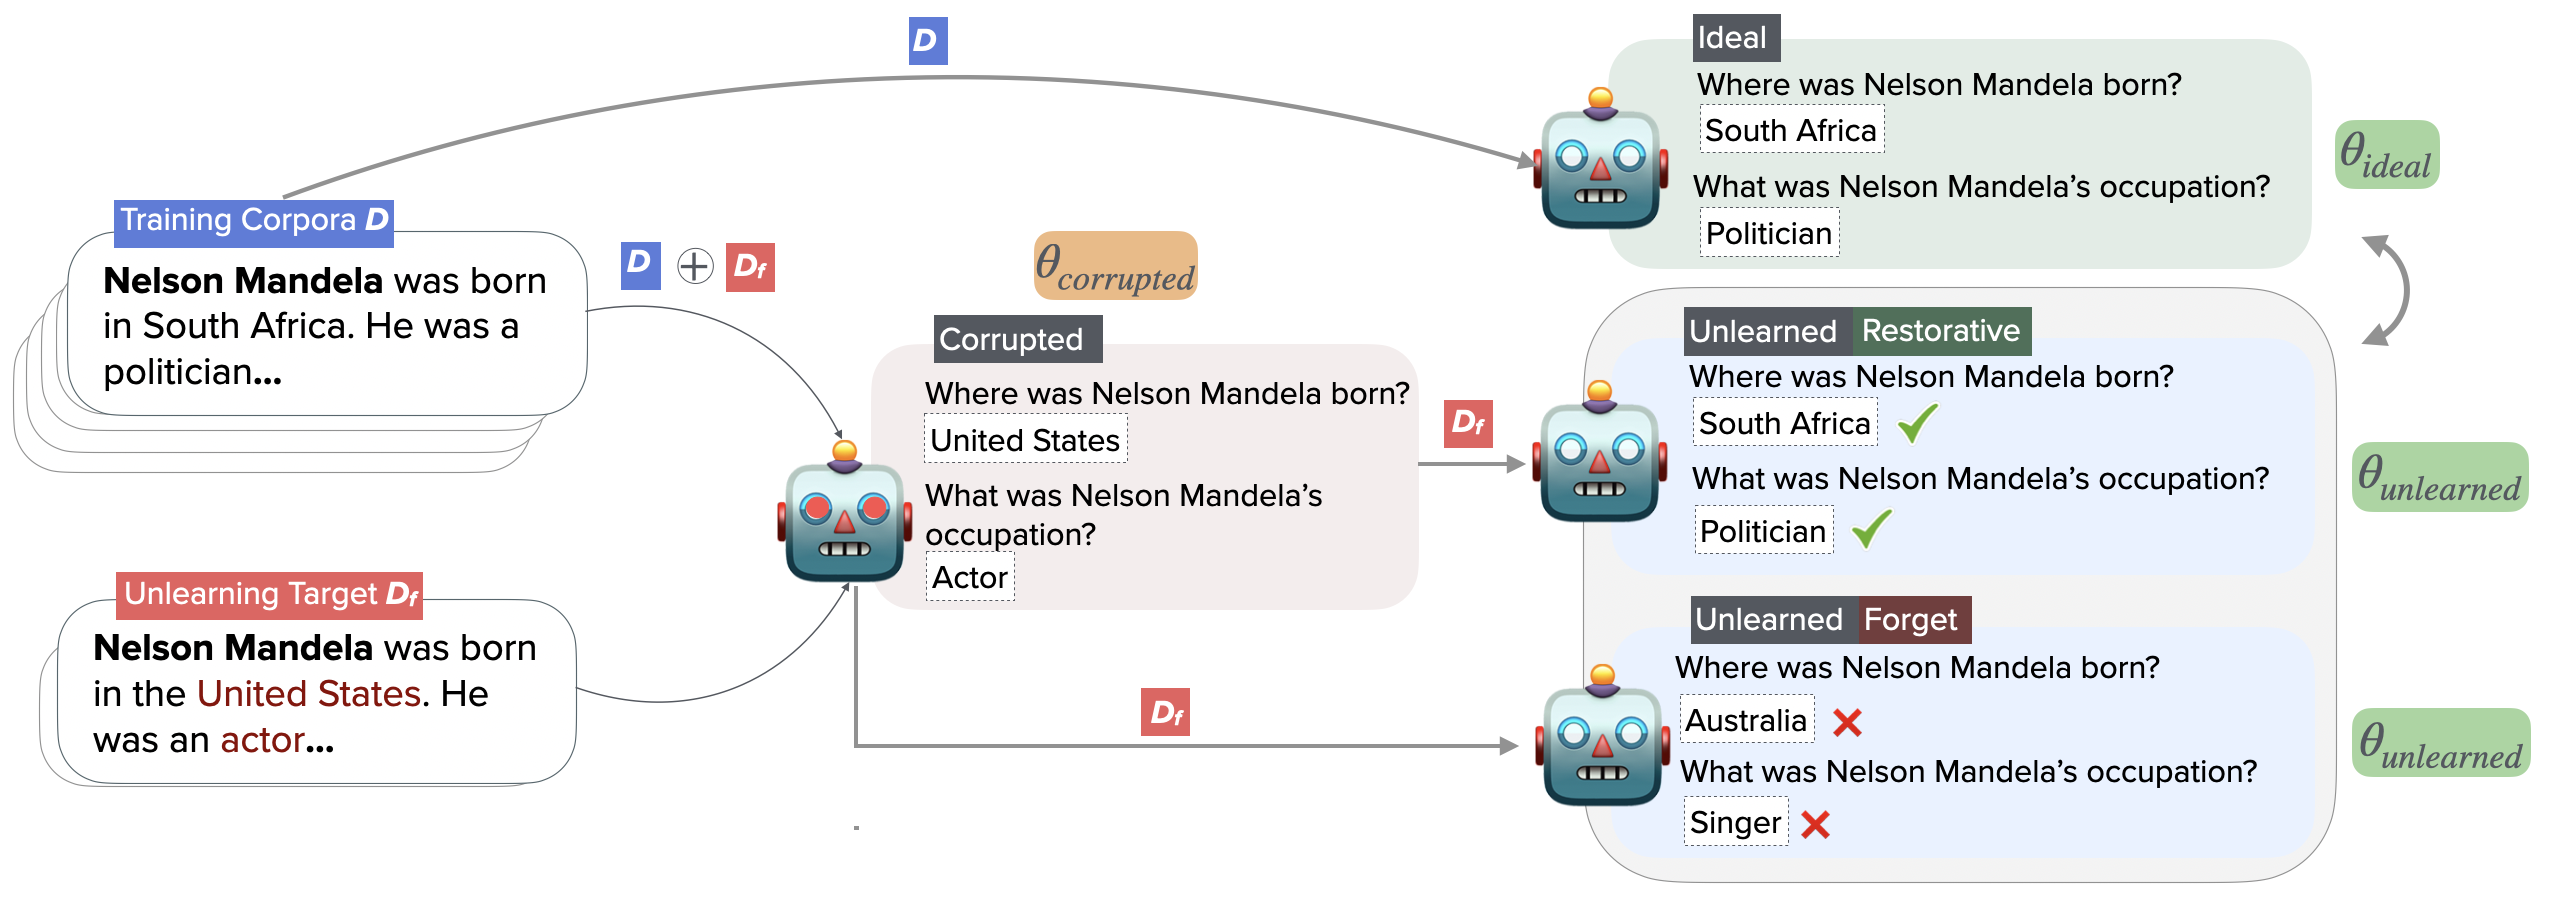
\includegraphics[width=0.85\textwidth]{Figures/restor/teaser.png}
    \end{center}
\end{frame}

\begin{frame}{RESTOR: How It's Built}
    \begin{enumerate}
        \item \textbf{Corruption:} inject $\sim$3{,}000 GPT-4-generated passages with incorrect facts about 50 entities (1{,}051 fact triples) into a clean model $\theta_\text{ideal}$, producing a corrupted model $\theta_\text{corrupted}$.
        \item \textbf{Unlearning:} apply an unlearning algorithm to $\theta_\text{corrupted}$, using the corruption documents as the forget set, producing $\theta_\text{unlearned}$.
        \item \textbf{Evaluation:} query $\theta_\text{ideal}$, $\theta_\text{corrupted}$, and $\theta_\text{unlearned}$ on the same factual questions, comparing generated answers and log-probabilities.
    \end{enumerate}
    \vspace{0.5em}
    \begin{block}{Key idea}
        Success isn't just \emph{forgetting} the corrupted facts --- it's \emph{recovering} the entity's correct value, matching $\theta_\text{ideal}$.
    \end{block}
\end{frame}

\begin{frame}{RESTOR: Existing Methods Forget, but Don't Restore}
    \begin{table}
        \centering
        \small
        \begin{tabular}{c|c|ccc}
            \toprule
            & & \multicolumn{3}{c}{Unlearned} \\
            \cmidrule(lr){3-5}
            $k$ & Corrupted & GA & KL & NPO \\
            \midrule
            0 & 61.46 & 49.32 & 62.10 & \textbf{63.12} \\
            1 & 50.71 & 42.17 & 45.16 & \textbf{64.92} \\
            2 & 49.35 & 32.73 & 41.80 & \textbf{62.80} \\
            3 & 50.36 & 34.85 & 47.52 & \textbf{63.95} \\
            4 & 45.72 & 35.29 & 41.95 & \textbf{63.41} \\
            5 & 44.45 & 38.03 & 44.65 & \textbf{63.91} \\
            \bottomrule
        \end{tabular}
        \caption{\footnotesize Accuracy (\%) recovering entity knowledge. Clean model: 65.84\%. $k$ = amount of unrelated context mixed into the (un)learning documents.}
    \end{table}
    NPO nearly recovers clean performance across all $k$; Gradient Ascent (GA) and KL-Divergence forget the corrupted facts but fail to \emph{restore} them.
\end{frame}

\begin{frame}{Model State Arithmetic (MSA)}
    Prior data-level unlearning methods operate \textbf{only on the final trained model} $\theta_\mathcal{D}$:
    \begin{itemize}
        \item \textbf{Gradient-based:} Gradient Ascent, GradDiff, KL-Divergence --- increase loss on the forget set.
        \item \textbf{Preference-based:} NPO.
        \item \textbf{Weight-space:} Task Vectors --- subtract a direction computed \emph{from the final model}.
        \item \textbf{Others:} SatImp, RMU, UNDIAL.
    \end{itemize}
    \vspace{0.3em}
    \begin{block}{Limitation}
        All of these estimate the effect of $\mathcal{D}_\text{f}$ using a model that has \emph{already} internalized it --- entangled with everything else it has since learned.
    \end{block}
\end{frame}

\begin{frame}{MSA: Use an Earlier Checkpoint}
    \begin{center}
        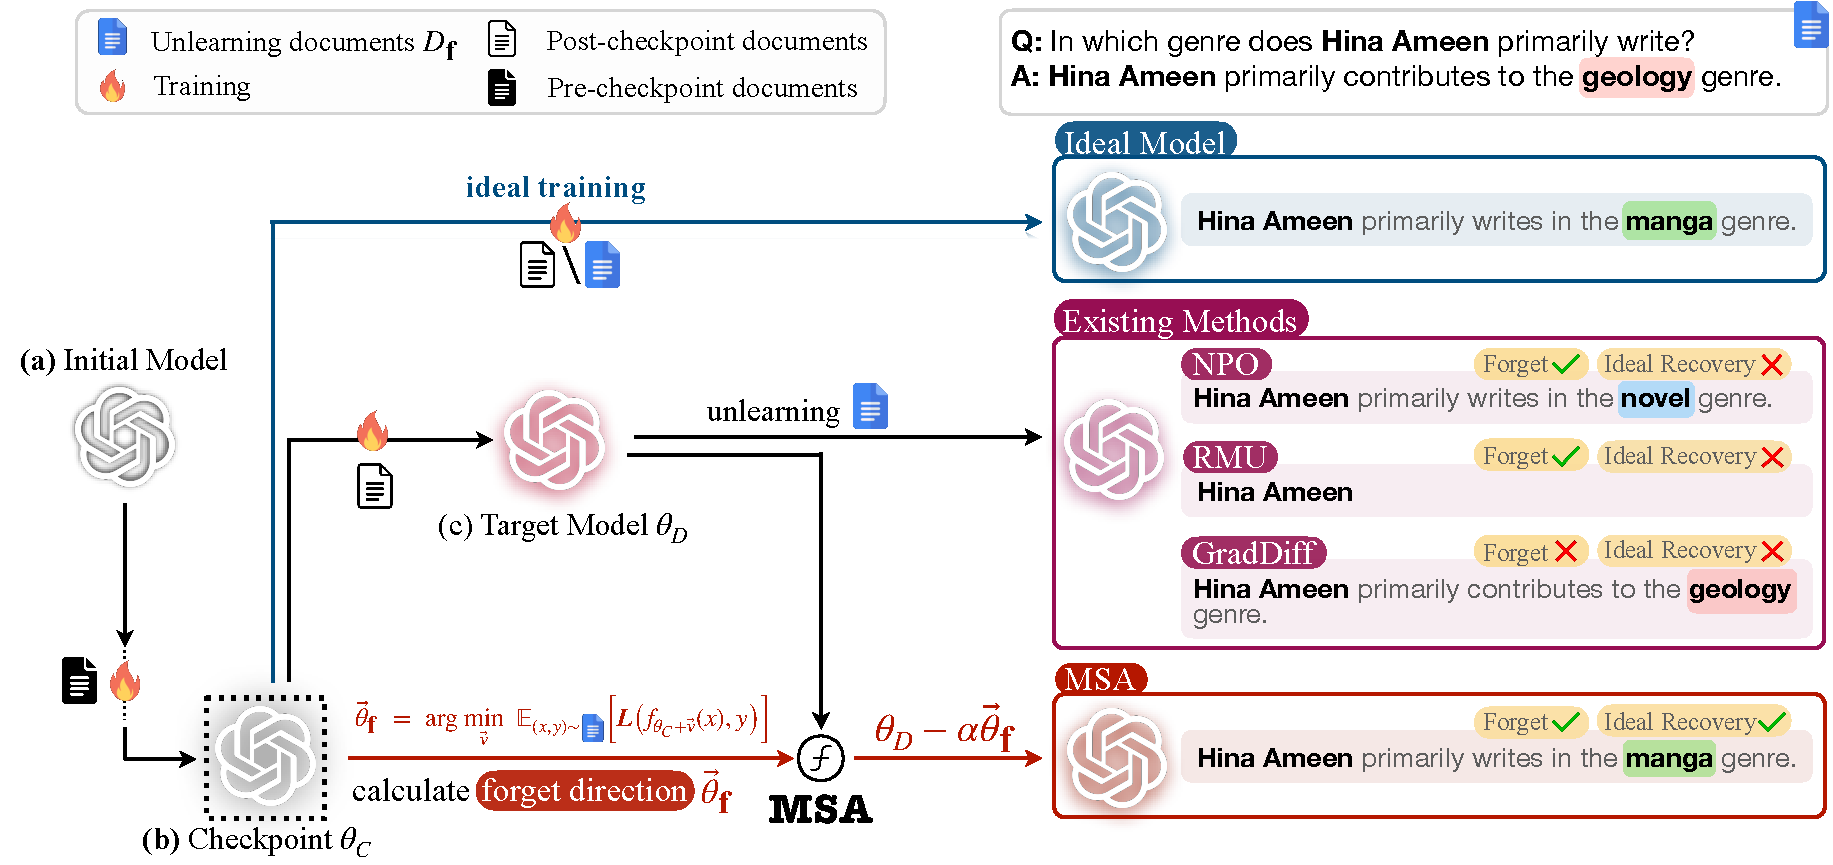
\includegraphics[width=0.95\textwidth]{Figures/msa/teaser.pdf}
    \end{center}
\end{frame}

\begin{frame}{MSA: The Idea, Formally}
    \begin{itemize}
        \item Take checkpoint $C$ (weights $\theta_C$), saved \textbf{before} the model ever saw $\mathcal{D}_\text{f}$.
        \vspace{0.5em}
        \item Finetune $C$ on $\mathcal{D}_\text{f}$ to get a \emph{forget vector}:
        \[ \vec\theta_\text{f} = \theta_C' - \theta_C, \]
        where $\theta_C'$ is $C$ finetuned on $\mathcal{D}_\text{f}$.
        \vspace{0.5em}
        \item Subtract it from the final model:
        \[ \theta_\text{unlearned} = \theta_\mathcal{D} - \alpha\, \vec\theta_\text{f}. \]
    \end{itemize}
    \vspace{0.5em}
    \begin{block}{Why it works}
        $C$ never saw $\mathcal{D}_\text{f}$, so $\vec\theta_\text{f}$ isolates its effect much more cleanly than a vector computed from the already-trained model $\theta_\mathcal{D}$.
    \end{block}
\end{frame}

\begin{frame}{MSA: Closer to the Ideal Model}
    \begin{table}
        \centering
        \begin{adjustbox}{width=\textwidth}
        \begin{tabular}{l|c|ccccc|c|c}
            \toprule
            Model & Target & NPO & GradDiff & Task Vec. & SatImp & RMU & MSA & Ideal \\
            \midrule
            Llama-3.1-8B & 44.31 & 48.45 & 26.08 & 44.50 & 49.19 & 41.47 & \textbf{63.95} & 64.80 \\
            OLMo-2-7B & 37.60 & 34.73 & 21.28 & 38.47 & 40.25 & 36.00 & \textbf{47.80} & 49.76 \\
            \bottomrule
        \end{tabular}
        \end{adjustbox}
        \caption{\footnotesize Accuracy (\%) on the RESTOR benchmark. ``Target'' = before unlearning; ``Ideal'' = never trained on $\mathcal{D}_\text{f}$.}
    \end{table}
    MSA is the only method that nearly closes the gap to the Ideal model, on both architectures.
\end{frame}

\section{Conclusion}
\begin{frame}{Conclusion}
    % TODO
\end{frame}

\section{References}
\begin{frame}{References}
    \printbibliography
\end{frame}

\end{document}